\documentclass[utf8]{article}
\usepackage{ctex}
\usepackage{graphicx}
\usepackage{float}
\usepackage{amsmath}
\usepackage{listings}
\usepackage{xcolor}
\usepackage{lipsum}
\usepackage{hyperref}

\title{\fontsize{18}\baselineskip Cache替换实验报告}
\author{王琛 \quad 计65 \quad 2016011360}
\date{}
\newcommand{\upcite}[1]{\textsuperscript{\textsuperscript{\cite{#1}}}}
\hypersetup{
    colorlinks,linkcolor=blue,anchorcolor=blue,citecolor=black,
} %set link in table of contents to black (default red)

\definecolor{vgreen}{RGB}{104,180,104}
\definecolor{vblue}{RGB}{49,49,255}
\definecolor{vorange}{RGB}{255,143,102}
\definecolor{light-gray}{gray}{0.97}
\lstset
{
	basicstyle={\footnotesize\ttfamily},        % set code style
	keywordstyle=\color{vblue},
	identifierstyle=\color{black},
	commentstyle=\color{vgreen},
	numbers=left,                      % set line numbers
	numberstyle={\tiny \color{black}}, % set fonts of line numbers
	frame=lines,                      % set type of open 
	numbersep=10pt,
	breaklines=true,                   % automatic line break
    tabsize=4,
    aboveskip=10pt,
    belowskip=2pt,
    backgroundcolor = \color{light-gray}
}
% \setlength\parindent{0pt} %default no indent

\begin{document}
\maketitle

\section{什么是Cache替换}
Cache是主存储器的高速缓存,当要访问的内容不再Cache中时,则需要将主存中相应的内容。由于容量有限,Cache中的一块可能对应多块相应大小的物理地址,装入时可能有多个可被替换的Cache块。而Cache的组织方式一般分为三种:全相连,多路组相连和直接映射。实际应用中基本采用多路组相连的方式,则Cache替换就是在多路中按照某种策略选择一路进行替换。不同的替换策略对于访存性能有着不同的影响。

\section{已有的不同Cache替换策略分析}
\subsection{Random}
Random算法就是在所有可供选择的Cache中随机选取一块进行替换。由于没有考虑程序的访存特征,Random算法对于相同的程序效果并不稳定。其优点在于实现简单,并且对于不同的极端情况也能够很好的适应。

\subsection{LRU}
LRU算法利用过去的访问行为推测未来,其基本思想是替换Cache块中最久没有被访问的。可以用类似堆栈的方式实现,每个块进行编号,当某个块被访问时,将所有小于该块的编号加1,该块编号置0;替换时选择编号最大的块。使用LRU算法,当程序展现出较好的局部性时,效果比较好。但是当程序执行扫描而Cache容量相对较小时,命中率比较低,因为前面的总是会被替换出去。

\subsection{LFU}
LFU是根据近期访问的频率来确定被替换的块,频率最低的会被替换出去。LFU也利用了程序的局部性特征,但是问题在于其容易替换掉刚刚被换进来的块。而且当程序切换到另一块访存空间时,原来的块由于访问次数多不容易被替换,导致刚切换很容易缺页。

\subsection{Protected LRU}
Protected LRU同时考虑访问次数和访问的时间。由于LRU替换访问时间早的块,那些之前访问次数多最近没有被访问的块很容易被替换掉,而这些块接下来很可能再次访问。因此,每次替换时,选择一定数目访问次数较多的块,设置为Protected,不会被置换;在剩下的块中选择最早被访问的替换。在本框架中,我进行了实现,每个Cache块记录访问次数,为了避免LFU的问题,最大次数设置为8次,每次替换时保护12个,从剩下的4个中选择最早使用的替换出去。

\subsection{LIP}
LIP算法与LRU的最大区别在于,当新的cache块被换入时,LIP将其放到LRU的位置,只有当再次被访问时,才将其放到MRU的位置。这样避免了新换入的块将原cache中的块挤出去。

\subsection{BIP}
BIP思路和LIP差不多,是将新换进的块随机放到MRU和LRU的位置。使用一个参数$\epsilon$,当随机的数比$\epsilon$大时,放到LRU,否则放到MRU。

\subsection{RRC}
RRC算法也是基于LIP的思路, 是17年新发表的一篇文章\cite{1}。当一个cache块被替换进来时,首先将其放到LRU的位置,只有当其被引用的次数到达某个阈值时将其挪到MRU的位置。如图所示:
\begin{figure}[H]
	\centering
	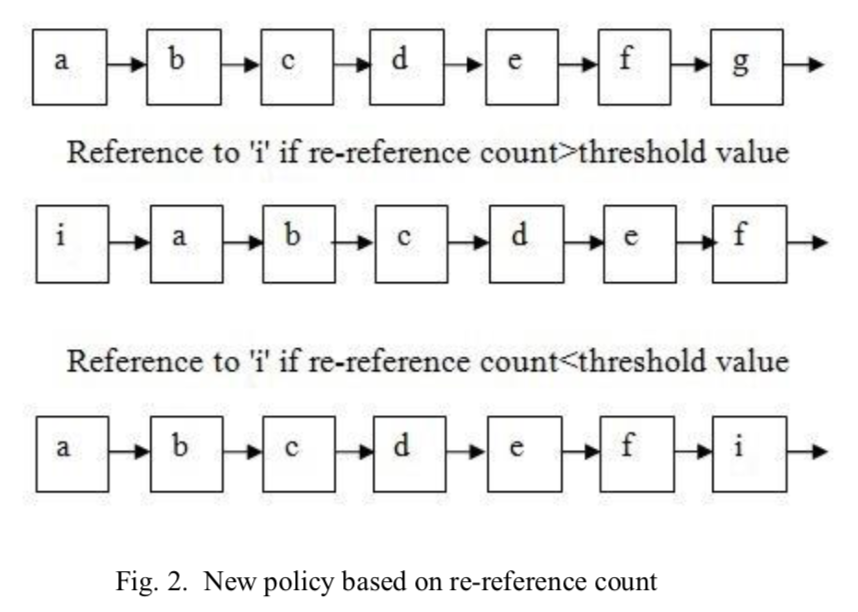
\includegraphics[scale=0.5]{./photos/rrc.png}
	\label{Fig1}
\end{figure}
我在本次实验中实现了这个算法,但是效果似乎并不理想。

\subsection{EHC}
EHC全称为Expected Hit Count,也是18年提出的\cite{3}。该算法的核心是一个cache块被重新使用的次数和其两次被重用的距离有关系。算法将相邻的四个块作为整体,记录他们在一段时间内的使用次数;然后据此推断下一次访问的间隔。选择victim时,选择下一次访问间隔最远的块。
\begin{figure}[H]
	\centering
	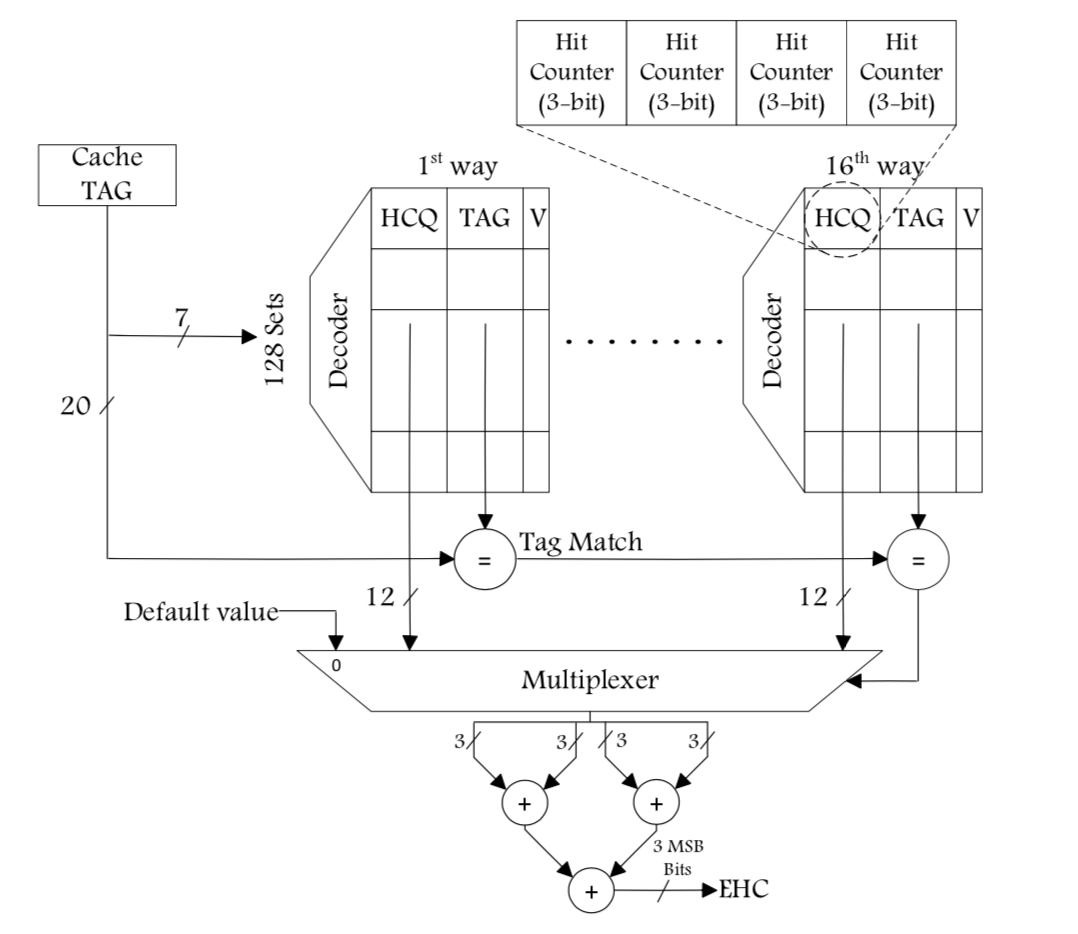
\includegraphics[scale=0.5]{./photos/ehc.png}
	\label{Fig1}
\end{figure}

\subsection{Score}
Score算法是Cache replacement championship中提出的算法\cite{2},思路是给每个块一个score,选择victim时从分数低于阈值的随机挑选。刚运行时,每个块的初始分数为最大分数的一半,每个阶段初始分数变化一个step,初始变化方向为增加。监控每个阶段的缺失率,如果当前缺失率大于之前的阶段,则改变初始分数变化的方向。访问某个块时,该块的score增加,其余的块score减小。

\section{新提出的Cache替换策略 -- WMBP}
我提出的Cache替换策略是Workset Miss Rate based Points policy (WMBP),是基于Score策略作出的改进。Score算法的问题在于无论是初始score的变化量还是选取victim的阈值都是一个绝对量,无法反应换入换出块在队列中的相对位置。因此如果前一阶段剩余块和当前阶段的分数绝对值相差较大时会出现问题。我的思路是给每个块一个point,根据一个Workset的缺失率确定初始point和victim的选择。下面具体阐述:
\subsection{初始point的选择}
Point的相对大小其实反映了LRU算法中的相对位置。当换入一个新的块时,无论是直接放入LRU的位置还是MRU的位置,在特殊的情况下性能都会很糟糕。之前的算法,无论是LRU, MRU, LIP, BIP放入时都没有考虑程序之前的访问特性。WMBP的思路是,如果当前工作集的缺失率越高,说明访存区域改变的可能性越大,因此新换入的块被用到的可能性更大,故应接近MRU的位置,即分数高;而当前如果缺失率很小,则新换进的块不适合放入LRU的位置,因为挤掉的块后续访问的可能性大,因此初始分数应该较低。具体实现时,找到队列中的maxPoint和minPoint,将minPoint+missRate*(maxPoint-minPoint)作为初始分数。此外,只有当工作集窗口大小到达最大窗口的某个比例才开始使用这种方法,否则直接将初始point设置最大point一半。这样做是为了防止窗口较小时发生抖动从而影响结果。代码如下:
\begin{lstlisting}[language=c++]
    if(5*numAccess > WINDOW_SIZE) {
        float missRate = float(curMiss)/float(numAccess);
            replSet[updateWayID].point = minPoint + int(missRate*(maxPoint-minPoint));
        } else {
            replSet[updateWayID].point = MAX_POINT >> 1;
        }
    }
\end{lstlisting}

\subsection{cache命中时数据的更新}
当cache命中时,被命中的块points要增加,而没有被命中的块point相对要减小。

\subsection{Victim的选择}
在Score算法中,Victim是通过固定阈值过滤的,这样做的问题是阈值对结果影响较大。可能出现同一阈值有的情况下全部过滤,有的情况一个也无法过滤。因此,在WMBP算法中,Victim有一个集合,从这个集合中挑选Victim,而这个集合的大小是动态变化的。同样,当前工作集的缺失率决定了集合大小如何变化。缺失率越高,这个集合越大,更多的块都可能被替换掉;缺失率低,只有少数的point小的被替换。这个思路实际上借鉴了PLRU,只是PLRU的Victim集合大小是固定的。实现时,将集合大小首先设置为定值,当缺失率大于一半时,增加集合大小;否则减小集合大小。同样和初始point选择一样,需要考虑当前窗口过小的问题。
\begin{lstlisting}[language=c++]
    if(5*numAccess > WINDOW_SIZE) {
        float missRate = float(curMiss)/float(numAccess);
        if(missRate > 0.5) {
            victimNum += missRate * 4;
        } else {
            victimNum -= missRate * 4;
        }
        if(victimNum > VICTIM_SET_MAXSIZE) victimNum = VICTIM_SET_MAXSIZE;
        if(victimNum < 1) victimNum = 1;
    }
\end{lstlisting}

\section{各种替换算法的比较}
本次实验中,我实现了PLRU, SCORE, RRC, WMBP算法,框架中已有LRU和Random。对这些算法进行了测试,其中RRC算法结果有些离谱,结果不再列出。测试环境为Ubuntu 10.04,使用了提供的29个benchmark,且测试时外部环境相同,没有其他运行的程序(实验证明这点对时间的测量影响较大)。Cache大小均为1024KB,16路组相连,每个块大小为64B。

每个算法在不同benchmark下的缺失率和运行时间见下图:
\begin{figure}[H]
	\centering
	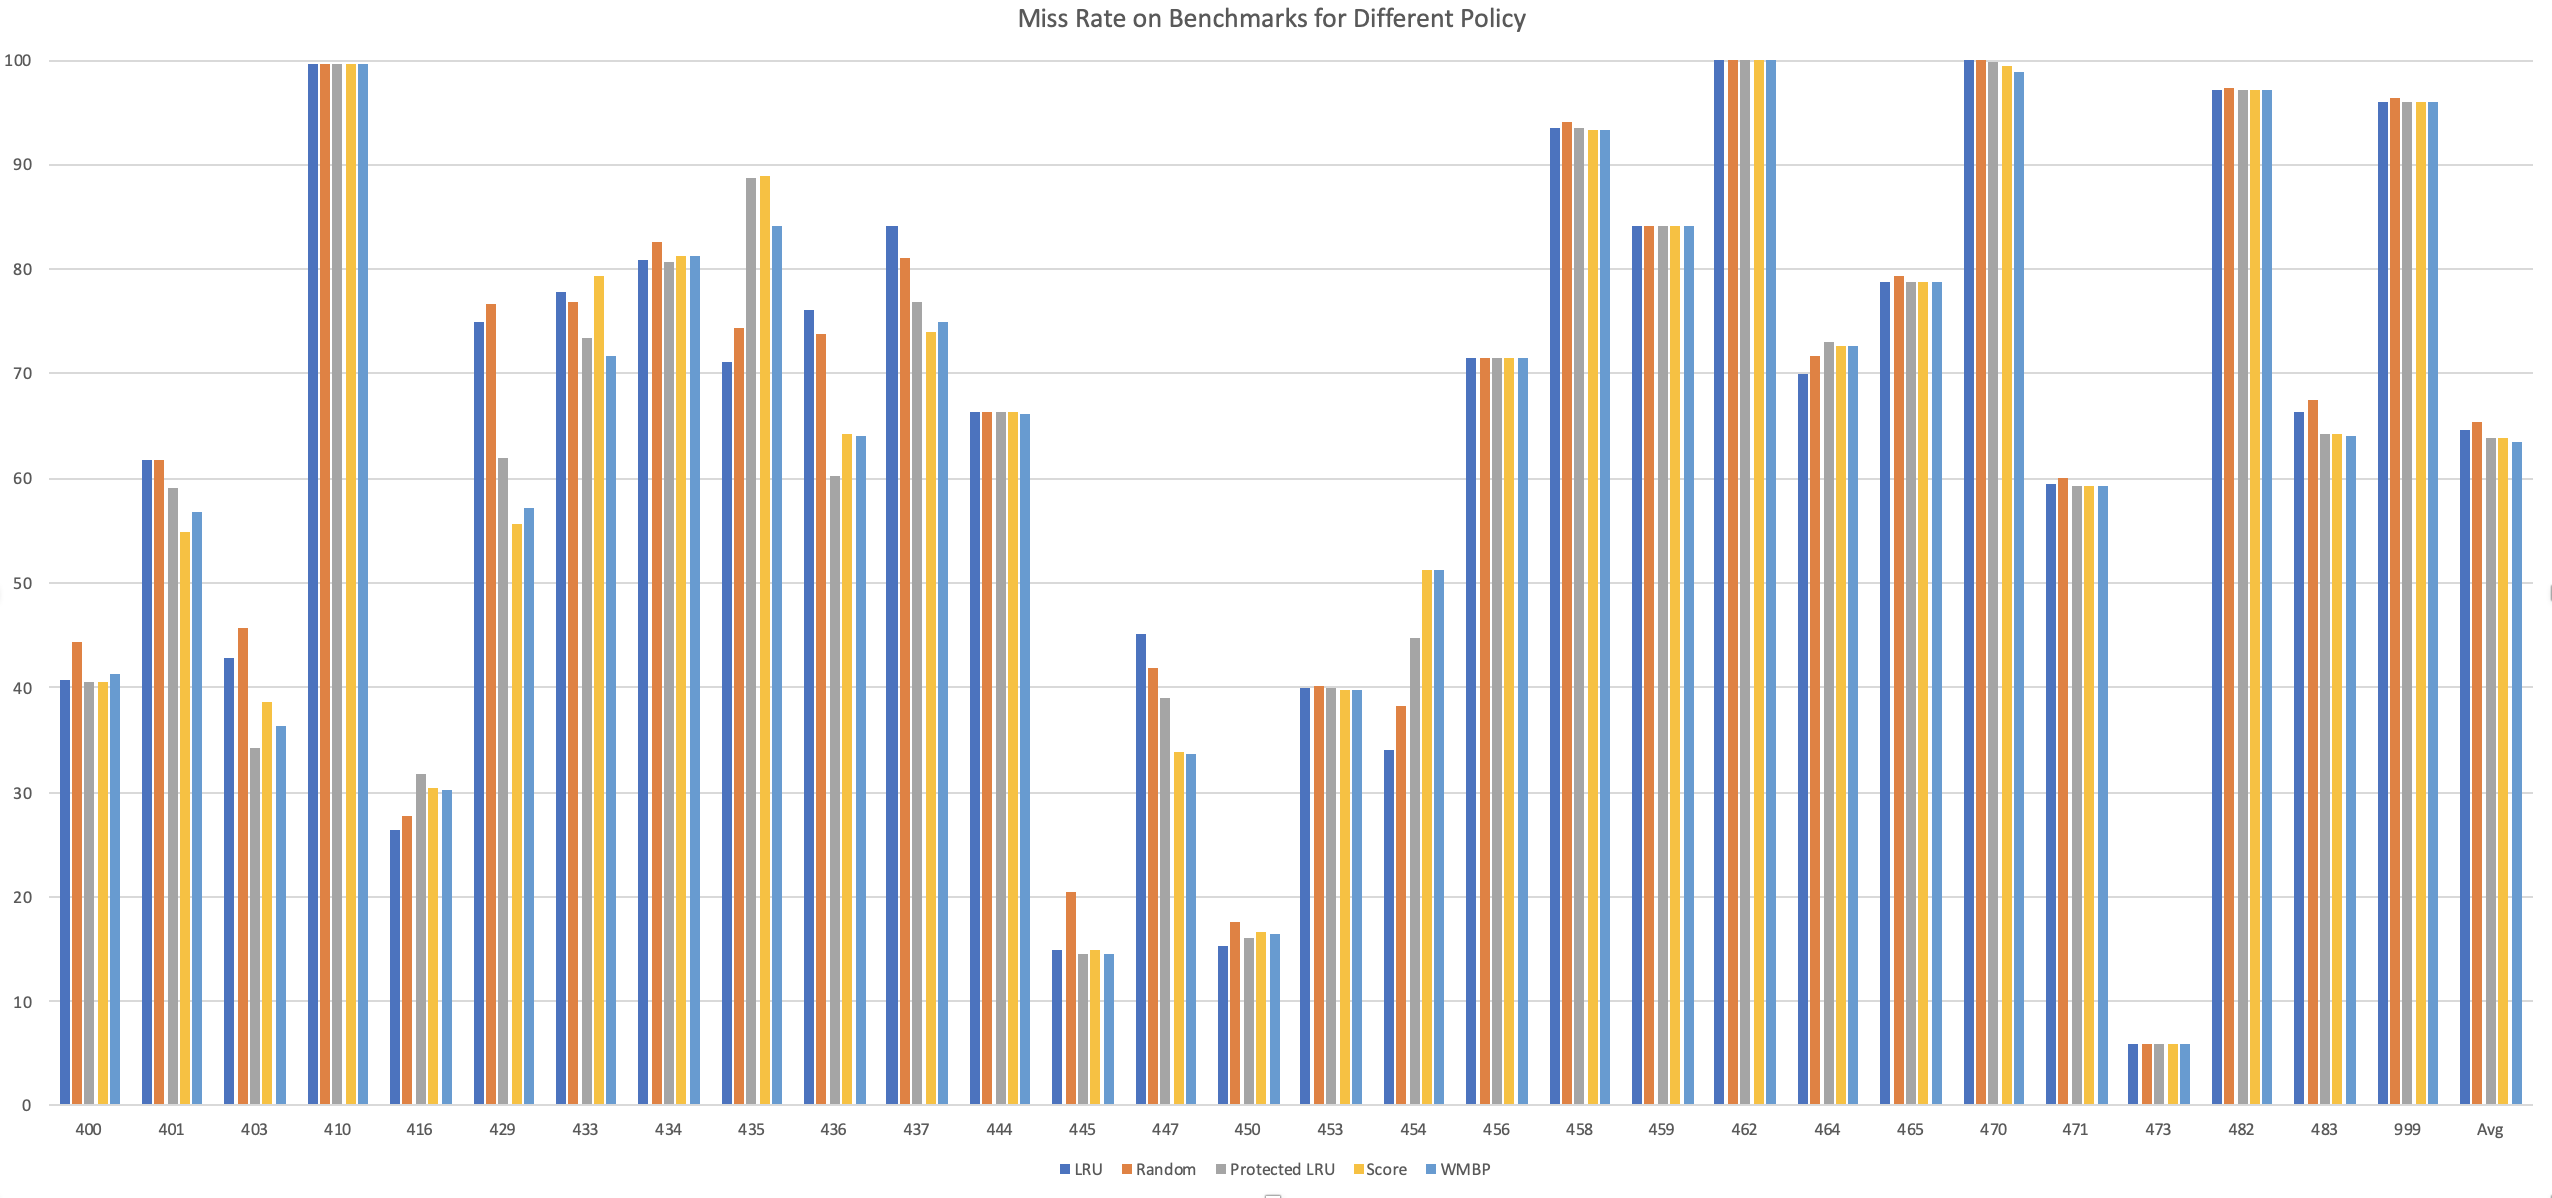
\includegraphics[scale=0.3]{./photos/mr.png}
    \label{Fig2}
    \caption{不同算法的缺失率}
\end{figure}

\begin{figure}[H]
	\centering
    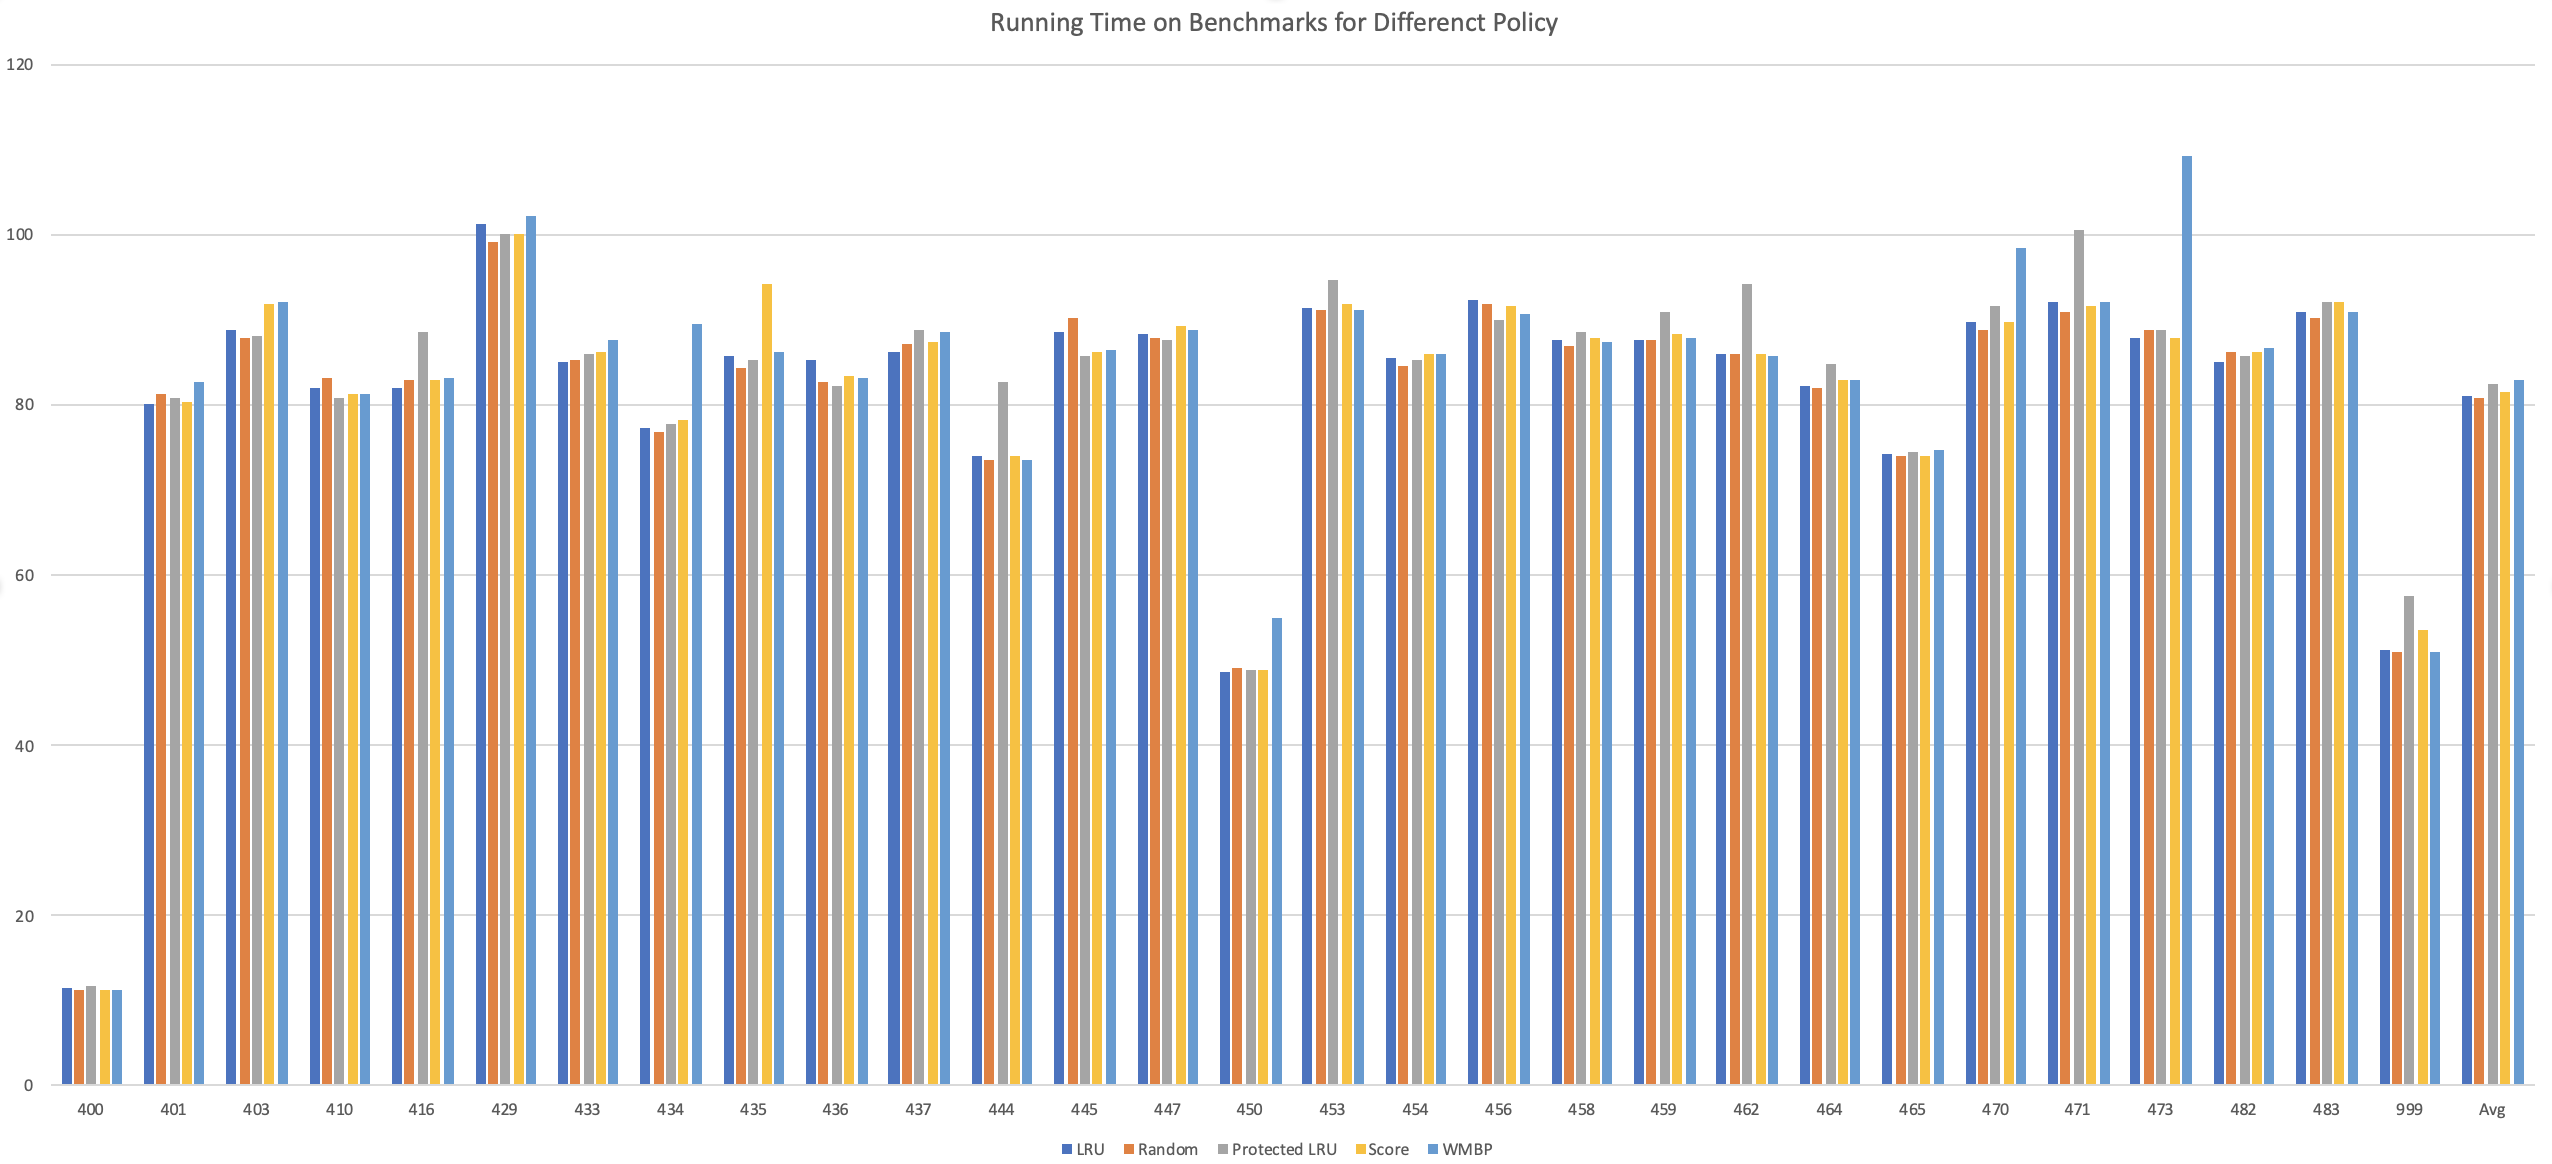
\includegraphics[scale=0.3]{./photos/time.png}
    \caption{不同算法的运行时间}
	\label{Fig3}
\end{figure}

分别比较WMBP和Score、LRU的缺失率:
\begin{figure}[H]
	\centering
    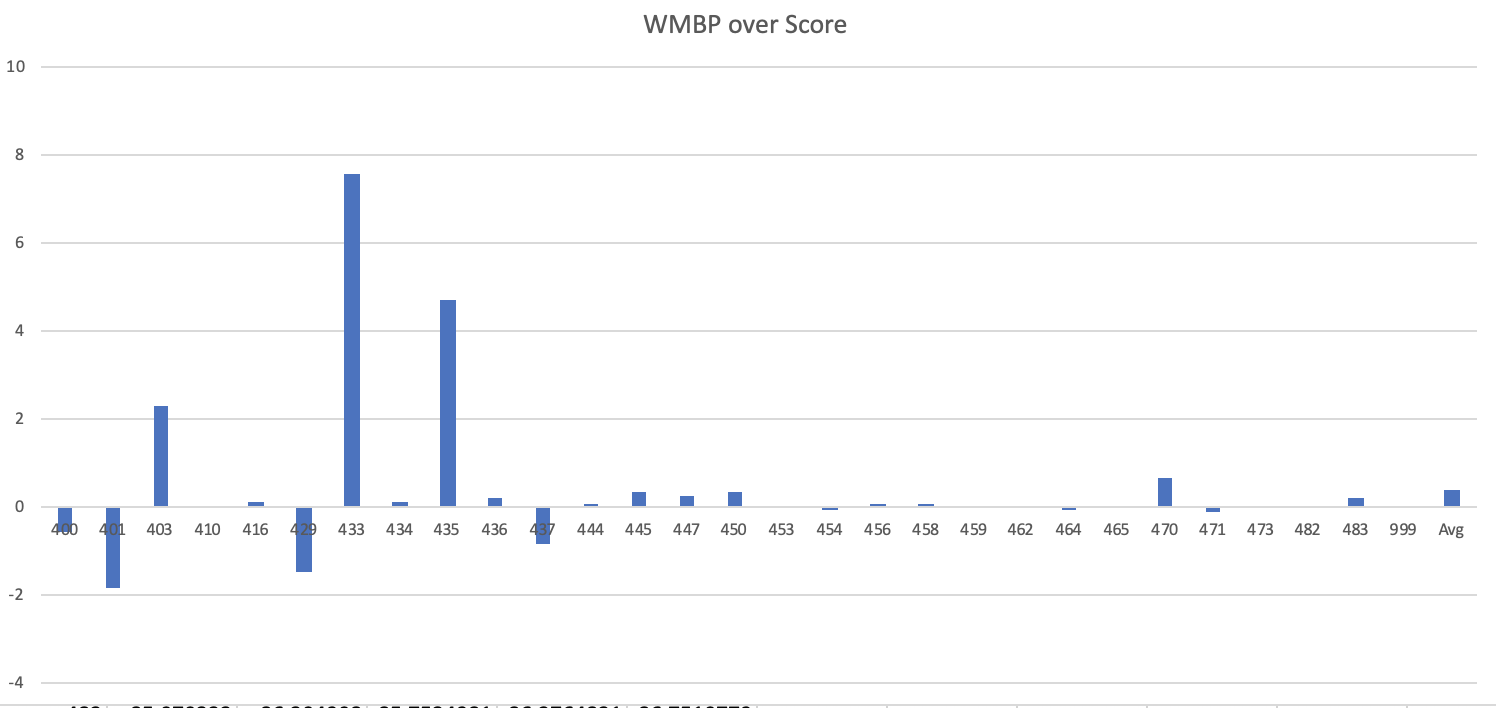
\includegraphics[scale=0.5]{./photos/score.png}
    \caption{WMBP over Score}
	\label{Fig3}
\end{figure}

\begin{figure}[H]
	\centering
    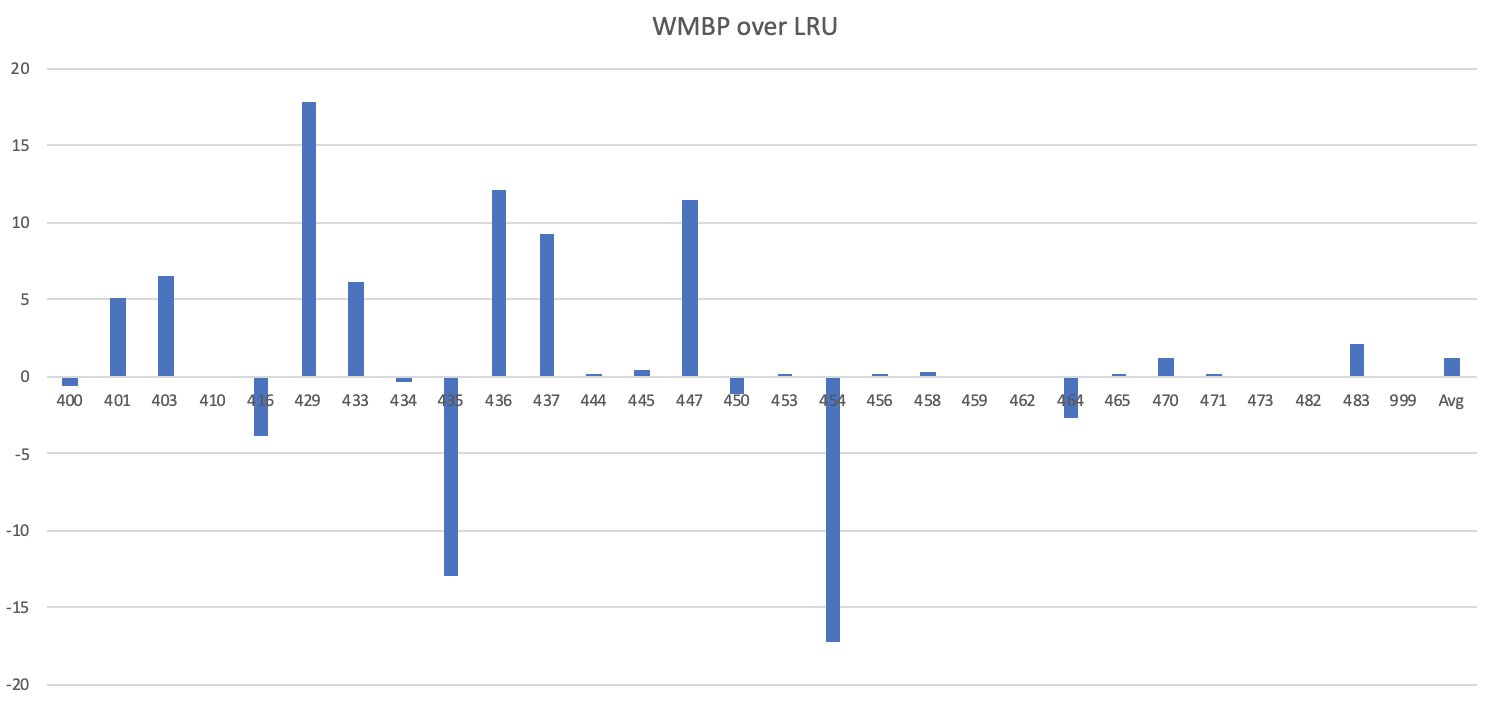
\includegraphics[scale=0.5]{./photos/lru.png}
    \caption{WMBP over LRU}
	\label{Fig3}
\end{figure}

\subsection*{结果分析}
从图中可以看出,不同的算法和baseline相比时,有的trace较好,有的trace较差。在大部分的算法下,缺失率WMBP < Score < PLRU < LRU < Random;平均下来也是如此。有些情况值得注意:
\begin{itemize}
    \item 416/435/454/464中Random算法比除了LRU之外的算法都要好。说明这些trace更加接近LRU的访存特征。
    \item 433/436/437/447中Random算法都要好于LRU算法,说明这些trace可能会继续使用未被替换的块,而LRU会将这些块优先换出,因此效果不好。
    \item 410/462/482/499这几个trace缺失率很高,所有的算法都难以改善;可能是因为程序几乎没有局部性,因此无法改善。
    \item 470这个trace在LRU/PLRU/Random算法下缺失率大于99.7,而Score将其降到了99.4,WMBP进一步降到了98.8。这个trace应该是cache刷新较快,使用LRU和PLRU很快会被替换出去,而Score和WMBP算法由于采用记分机制,原有的cache块不容易被替换,因此较好。而WMBP初始分值和换出策略还考虑了相对顺序,会更合理一些。
\end{itemize}

而对于不同替换的运行时间,平均而言WMBP > PLRU > Score > LRU > Random。和命中率一样,就平均而言其实相差并不大,但是在某些trace上相差比较明显。比如PLRU在444和462比其他要高很多;而WMBP在450和473高的很明显。这也是显而易见的,因为这两种算法都要首先选取一定大小的victim set,所以会消耗较多的时间。我原本认为WMBP会比其他几种算法消耗比较多的时间,但是在有些情况下时间消耗甚至比较少,我认为是局部性较好,从而victim set比较小,比如999,消耗时间较少而且准确率还比较高。

\subsection*{自己的trace}
我认为我设计的cache算法核心仍然是将新换入的块放到队列中的位置,LRU是放在MRU出,MRU是放在LRU处,BIP随机放置,而WMBP是根据缺失率动态调整位置。所以,假设cache只有4路,一般的LRU碰到abcdeabcde这样重复的访存序列,缺失率会趋向100\%,因为总是会将下一个要访问的块挤出去。类似这种序列在现有的几种算法(除了WMBP)效果都不好。而WMBP虽然不像MRU直接放到LRU位置,但是能动态适应,因此缺失率最低。比如下面的程序:
\begin{lstlisting}[language=c++]
    #include<iostream>
    using namespace std;
    int main(){
        int a[278528], i, j;
        for (i = 0; i < 10; i++) {
            for (j = 0; j < 278528; j++) { 
                a[j] = i + j;
            } 
        }
        return 0;
    }
\end{lstlisting}
将其制作成trace,结果如下:
\begin{center}
	\begin{tabular}{lcc}
        \hline  
        Policy & Miss Rate & Running Time \\  
        \hline  
        WMBP & 30.74 & 25.49 \\
        \hline
        Random & 34.05 & 24.31 \\  
        \hline  
        PLRU & 51.99 & 26.71 \\
        \hline
        LRU & 99.83 & 28.85\\
        \hline
        Score & 32.66 & 31.03\\
        \hline
	\end{tabular}
\end{center}
这段程序是专门针对本次实验所采用的cache设计的,循环访问a数组,a数组的大小正好比cache多一路。如果采用LRU算法,每次都会缺失;而PLRU会保护刚刚访问的,由于每个block有8个int,很快被再次访问,因此缺失率将近一半;这种情况Random反而效果较好,因为不容易将下次要访问的挤出去;而Score和WMBP使用计分算法,而WMBP还考虑了缺失率和相对位置,因此缺失率最低;时间也仅次于Random。

\subsection*{WMBP算法优缺点分析}
WMBP的优点是显而易见的,克服了LRU一类算法可能出现的问题,并且在LRU表现较好的情况下效果仍然很好。由于将计分策略和缺失率相结合,算法能够比较好的随着程序访存特性变化,因此总体的缺失率也比较低。

当然,WMBP实现有些复杂,需要记录较多的变量,而且涉及到浮点运算,所以运行时间较长,不过仍然在可接受范围之内。另外,此算法在片上可能难以实现,只能停留在模拟器阶段。

\section{实验总结}
本次实验,我对于不同的cache替换策略有了一个初步的认识,也阅读了竞赛的论文和近年的几篇论文。虽然cache替换策略并不是一个新的话题,但是仍然保持着一定的活力。另外,在实验中,我也体会到了没有一个完美的cache替换策略,每种方法都有不适用的情形。

\begin{thebibliography}{1}
    \bibitem{1} Sreedharan, S., \& Asokan, S. (2017, March). A cache replacement policy based on re-reference count. In 2017 International Conference on Inventive Communication and Computational Technologies (ICICCT) (pp. 129-134). IEEE.
    \bibitem{2}  Nam, D., Rosario C., etc. SCORE: A Score-Based Memory Cache Replacement Policy
    \bibitem{3} Vakil-Ghahani, A., Mahdizadeh-Shahri, S., Lotfi-Namin, M. R., Bakhshalipour, M., Lotfi-Kamran, P., \& Sarbazi-Azad, H. (2018). Cache replacement policy based on expected hit count. IEEE Computer Architecture Letters, 17(1), 64-67.
\end{thebibliography}

\end{document}
